\section{Theorie}
\label{sec:Theorie}

\subsection{Zielsetzung}
\label{subsec:zielsetzung}
Ziel des im Folgenden beschriebenen Versuchs ist es,
mit Hilfe des Prinzips der Röntgenreflektrometrie
einen Nanometer-dicken Polystyrolfilm, der auf einen Silizium
Wafer aufgetragen ist, zu untersuchen.
Dazu wird ein D8-Labordiffraktometer zunächst justiert und anschließend zu
Messungen verwendet, aus deren Ergebnissen dann Schichtdicke, Rauigkeit und
Elektronendichte der Probe, sowie des Siliziumwafers bestimmt werden.


\subsection{Brechung von Röntgenstrahlung an einer Grenzfläche}
\label{subsec:einschicht}
Um das Prinzip der Röntgenreflektrometrie zu verstehen ist es notwendig,
sich mit der Brechung von Röntgenstrahlung an einer Grenzfläche auseinander
zu setzen.
% Brechungsindex
Bei Röntgenstrahlung handelt es sich um elektromagnetische Wellen, deren
Wellenlängen in einem Bereich von circa $\SI{0.1}{\angstrom}$ bis
$\SI{10}{\angstrom}$ liegen.
Um den Übergang einer solchen Welle von einem Medium mit Brechungsindex $n_{1}$
in ein zweites mit Brechungsindex $n_{2}$ (siehe Abbildung \ref{fig:einschicht})
zu beschreiben, kann das Brechungsgesetz nach Snellius
\begin{align}
  n_{1} \cos\alpha_{\text{i}} = n_{2} \cos\alpha_{\text{t}}
  \label{eqn:snellius}
\end{align}
verwendet werden. Dabei bezeichnet $\alpha_{\text{i}}$ den Einfallswinkel
und $\alpha_{\text{t}}$ den Winkel unter dem die Strahlung gebrochen wird
(vgl. Abbildung \ref{fig:einschicht}). Es wird eine ideale glatte Grenzfläche
angenommen. \\

\FloatBarrier
\begin{figure}
  \centering
  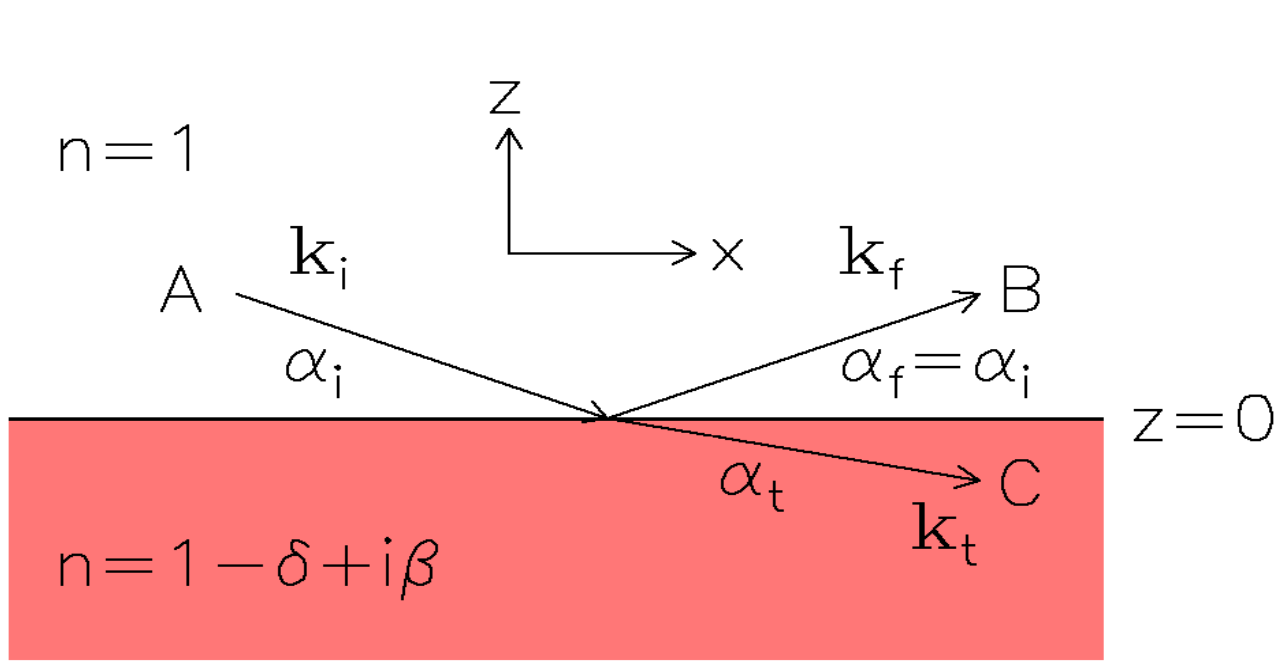
\includegraphics[width=0.7\textwidth]{bilder/einschicht.png}
  \caption{Übergang einer elektromagnetischen Welle vom Vakuum in ein
            anderes Medium und dabei auftretetende Reflexion und Transmission.\cite{sample}}
  \label{fig:einschicht}
\end{figure}
\FloatBarrier

In Abbildung \ref{fig:einschicht} wird für das Ursprungsmedium das Vakuum gewählt,
sodass gilt $n_{1} = 1$. Für den Brechungsindex $n_{2}$ des anderen Mediums,
wird eine komplexe Zahl
\begin{align}
  n_{2} = \alpha + i \beta& &\text{mit } \alpha, \beta \in \mathbb{N}
  \label{eqn:komplexerindex}
\end{align}
gewählt. Der Realteil $\alpha$ beinhaltet die Informationen bezüglich der
eigentlichen Brechung und der Imaginarteil $\beta$
die Dämpfung der Welle im Medium. Für Röntgenstrahlung gilt typischerweise
$\alpha < 1$. Dies liegt daran, dass der reele Brechungsindex das Verhältnis
von Lichtgeschwindigkeit im Medium zu der im Vakuum misst und für
Röntgenstrahlung die Phasengeschwindigkeit im Medium schneller
sein kann als die Vakuumlichtgeschwindigkeit $c_{0}$.
Da der Realteil von $n$ den Wert $1$ nur um sehr kleine Werte
$\delta \sim 10^{-6}$ unterschreitet, wird die Formulierung
$\alpha = 1 - \delta$ gewählt,
sodass aus Gleichung \eqref{eqn:komplexerindex},
\begin{align}
  n_{2} = 1 - \delta + i \beta
  \label{eqn:komplexerindexdelta}
\end{align}
wird.

% kritischer Winkel
Anhand des Brechungsgesetzes \eqref{eqn:snellius} wird klar , dass ein Winkel
$\alpha_\text{{crit.}} = \arccos\left( n_{2} \right)$ existiert,
unter dem die Welle nicht mehr in das zweite Medium eintritt,
also total refelektiert wird.
Damit überhaupt transmittierte Strahlung auftritt, muss also gelten,
$\alpha_{\text{i}} > \alpha_{\text{crit.}}$.\\
Wird der Imaginarteil von $n_{2}$ vernachlässigt und eine Entwicklung
des Kosinus in Gleichung \eqref{eqn:snellius} für kleine Winkel in
quadratischer Ordnung durchgeführt, so ergibt sich für den kritischen Winkel
\begin{align}
  \alpha_{\text{crit.}} \approx \sqrt{2 \delta} = \lambda \,
  \sqrt{\frac{ \rho \, r_{\text{e}} }{ \pi }} \, .
  \label{eqn:elektronendichte}
\end{align}
Dabei entpricht $\lambda$ der Wellenlänge der Strahlung, $\rho$ der
Volumendichte der Elektronen im Probenmaterial und $r_{\text{e}}$ dem
(klassischen) Elektronenradius.

% fresnel -> transmissions/reflektions amplituden -> Fresnelreflektivitaet
Wie bereits erwähnt und in Abbildung \ref{fig:einschicht} gezeigt,
entsteht bei der Interaktion einer elektromagnetischen Welle,
mit Wellenvektor $k_{\text{i}}$ mit einer dünnen Schicht im Allgemeinen
neben einer reflektierten Welle,
mit dem Wellenvektor $k_{\text{f}}$, auch eine transmittierte mit dem
Wellenvektor $k_{\text{t}}$ auf.
Die verschiedenen (elektrischen) Feldvektoren
$\vec{E}_{\text{index}}\left( \vec{r} \right)$
lassen sich wie folgt angeben.
Für die einlaufende Welle
$\vec{E}_{\text{i}} = \begin{pmatrix} 0, A, 0 \end{pmatrix}^{\top}
e^{ \i \vec{k}_{\text{i} \vec{r} }}$,
die reflektierte\\
$\vec{E}_{\text{f}} = \begin{pmatrix} 0, B, 0 \end{pmatrix}^{\top}
e^{ \i \vec{k}_{\text{f} \vec{r} }}$
und die transmittierte
$\vec{E}_{\text{t}} = \begin{pmatrix} 0, C, 0 \end{pmatrix}^{\top}
e^{ \i \vec{k}_{\text{t} \vec{r} }}$. \\
Dabei gilt für die Wellenvektoren
\begin{align*}
  \vec{k_{\text{i}}} &= k
  \begin{pmatrix}  \cos\alpha_{\text{i}} , 0, -\sin\alpha_{\text{i}} \end{pmatrix}^{\top}\\
  \vec{k_{\text{f}}} &= k
  \begin{pmatrix}  \cos\alpha_{\text{i}} , 0, \sin\alpha_{\text{i}} \end{pmatrix}^{\top}\\
  \vec{k_{\text{t}}} &= n \, k
  \begin{pmatrix} \cos\alpha_{\text{t}} , 0, -\sin\alpha_{\text{t}} \end{pmatrix}^{\top} \, .
\end{align*}

Hier wurde verwendet, dass bei Röntgenstrahlung nicht zwischen s- und p-Polarisation
unterschieden werden muss.

Anhand der vorausgegangenen Definitionen für die Feldvektoren sowie
Stetigkeitsbedingungen an den Grenzflächen, lassen sich die
fresnelschen Formeln %für senkrecht polarisierte Strahlung
\begin{align}
  r &= \frac{B}{A} = \frac{k_{\text{i,}z} - k_{\text{t,}z}}{k_{\text{i,}z} + k_{\text{t,}z}}\\
  \label{eqn:fresnel_r}
  &\intertext{und}
  t &= \frac{C}{A} = \frac{2 k_{\text{i,}z} }{k_{\text{i,}z} + k_{\text{t,}z}}
  \label{eqn:fresnel_t}
\end{align}
für den Reflektionskoeffizienten $r$ und den Transmissionskoeffizienten $t$
gewinnen.

Die Reflektivität $R$ bezeichnet das Verhältnis der reflektierten Intensität
zur eingestrahlten Intensität.
Das Betragsquadrat der
Feldstärke\footnote{Das Verhältnis der Feldstärken von einlaufender und
reflektierter Welle wird durch $r$ bemessen.} dient als Maß für die Intensität,
sodass sich die Reflektivität durch
\begin{align}
  R = \lvert r \rvert^{2} \approx
  \left( \frac{\alpha_{\text{crit.}}}{2\alpha_{\text{i}}} \right)^{4}
  \label{eqn:reflektivitaet}
\end{align}
ausdrücken lässt.\\
Die Näherung in Gleichung \eqref{eqn:reflektivitaet} ist für
$\alpha_{\text{i}} > 3\alpha_{\text{crit.}}$ vertretbar. Dabei ist zu erkennen,
dass diese (Fresnel-)Reflektivität mit der vierten Potenz von $\alpha_{\text{i}}$
abfällt.

% dag
\subsection{Brechung von Röntgenstrahlung in Mehrschichtsystemen}
\label{subsec:mehrschicht}
Im Folgenden wird nun nicht mehr
die Röngenreflektivität
eines einschichtigen
Mediums betrachtet, sondern eines Mehrschichtsystem wie
beispielsweise ein $\SI{800}{\angstrom}$ dicker Polystyrolfilm (PS)
auf Silizium (Si). Die berechnete Röngenreflektivität dieses
Systems ist in der Abbilung \ref{fig:mehrschicht} dargestellt.

\begin{figure}
\centering
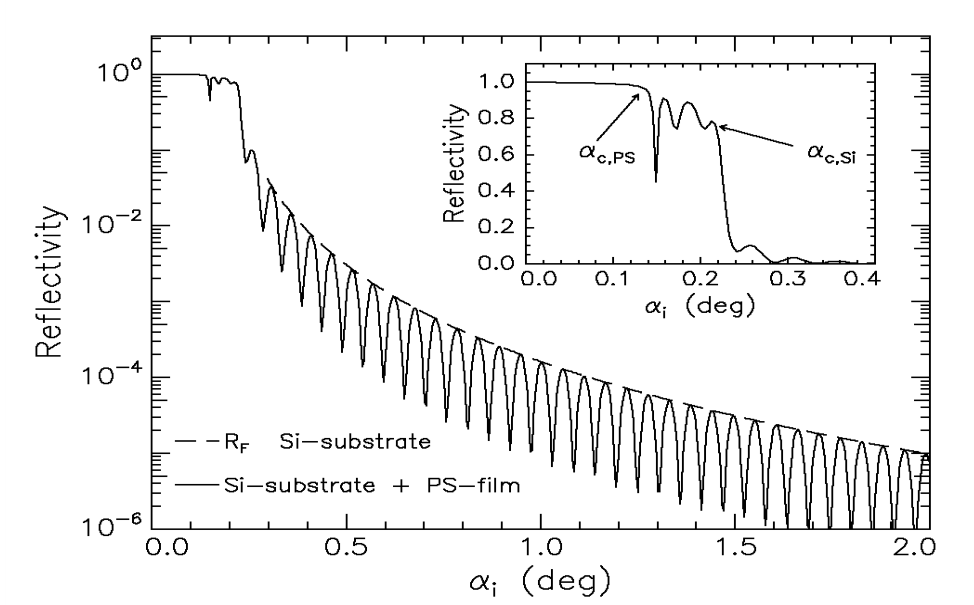
\includegraphics[width = 0.7\textwidth]{bilder/mehrschicht_beispiel.PNG}
\caption{Berechnete Röngenreflektivität für $\lambda=\SI{1.54}{\angstrom} $ sowohl
für einen $\SI{800}{\angstrom}$ dicker Polystyrolfilm (PS)
auf Silizium (Si)} als auch die reine Röngenreflektivität von Si ohne Film.
in Abhängigkeit des Einfallswinkel $\alpha_i$.\cite{sample}
\label{fig:mehrschicht}
\end{figure}

Deutlich zu erkennen ist der Abfall in der Reflektivität wie schon
bei einem Einschichtsystemen nach der Formel \eqref{eqn:reflektivitaet}.

Die Ozillationen in der Reflektivität aus Abbildung \ref{subsec:mehrschicht}
lassen sich auf konstruktive und destruktive Interferenzen
der refelektiert Strahlung zurückführen.
Da bei einem Mehrschichtsystem mehr
Grenzflächen, an denen Reflexion auftritt, existieren,
kommt es zu einer Überlagerung der an unterschiedlichen Grenzflächen
refelektierten Strahlen.
Beträgt der Gangunterschied der Strahlen
ein ungerades Vielfaches der halben Wellenlänge
kommt es zu destruktiver Interferenz und für gerade Vielfache
liegt konstruktive Interferenz vor.
Die so auftretetenden
Modulationen in der Reflektionskurve
werden auch "Kiessig-Ringe" gennant.
Für ein einfaches Modell mit zwei
Grenzschichten mit Schichtabstand $d$
ergibt sich der Zusammenhang
\begin{align}
  d = \frac{2\pi}{\Delta q_z} \approx \frac{\lambda}{2\Delta \alpha_i}. \label{eqn:schichtabstand}
\end{align}
Dabei ist $q$ der Wellenvektorübertrag, für den gilt
$\vec{q} = \vec{k}_f \vec{k}_i$ und welcher die z-Komponente $q_z=2k\sin \alpha_i$ besitzt.
Dabei sind $\Delta q_z$ und $\Delta\alpha_i$ Differenzen
der jeweiligen
Werte zwischen zwei benachbarten Minima. % ????????

Für Mehrschichtsysteme mit Schichten
unterschiedlicher Brechungsindizes
ergibt sich auf Grund der Überlagerungen der reflektierten
Strahlen eine
komplizierte Reflektivität, für die der
rekursive Parratt-Algorithmus einen Lösungsansatz
liefert.
Der Parratt-Algorithmus geht, wie in Abbildung \ref{fig:parratt_syst} dargestellt, von einem System
mit $N$ ideal glatten Grenzflächen und somit $N+1$ Schichten aus.

\begin{figure}
  \centering
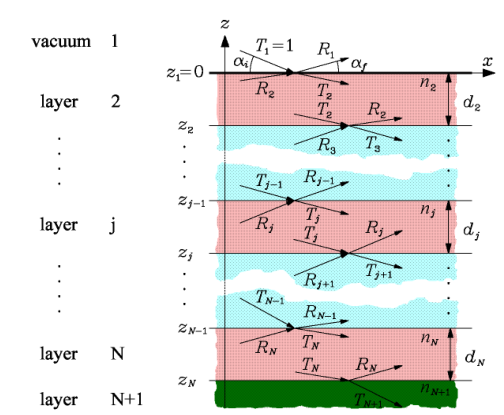
\includegraphics[width=0.7\textwidth]{bilder/mehrschicht_parratt.PNG}
\caption{Beispielsystem für den Parratt-Algorithmus
mit $N+1$ Schichten und $N$ glatten Grenzflächen.\cite{sample}}
\label{fig:parratt_syst}
\end{figure}

Die erste Schicht ist das Vakuum mit Brechungsindex $n=1$
und die letzte Schicht ist das Substrat, welches als
unendlich dick angenommen wird.
Diese Annahme ist
eine gute Nährung
solange
die Substratdicke groß gegenüber der
Eindringtiefe ist.
Als Folge dessen existiert ein Startwert
für den Parratt-Algorithmus, da
aus dem Substrat keine refektierte Strahlung $R_{N+1}$
existiert.
Für das Verhältnis von refelektierter und transmittierter Amplitude
$\mathrm{X}_j$ an der $j$-ten Grenzfläche liefert der
Parratt-Algorithmus den Zusammenhang

\begin{align}
\mathrm{X}_j = \frac{\mathrm{R}_j}{\mathrm{T}_j} = \exp\left(-2\symup{i} \mathrm{k}_{z,j} \mathrm{z}_j\right)
\frac{\mathrm{r}_{j,j+1} + \mathrm{X}_{j+1}\exp\left(2\symup{i} \mathrm{k}_{z,j+1} \mathrm{z}_j \right)}
{1 + \mathrm{r}_{j,j+1} + \mathrm{X}_{j+1}\exp\left(2\symup{i} \mathrm{k}_{z,j+1} \mathrm{z}_j \right)}.
\end{align}
Der Koeffizient $\mathrm{r}_{j,j+1}$ entspricht dabei
der Fresnelreflektivität an der $j$-ten Grenzfläche
mit
\begin{align}
  \mathrm{r}_{j,j+1} &= \frac{\mathrm{k}_{z,j}-\mathrm{k}_{z,j+1}}{\mathrm{k}_{z,j} + \mathrm{k}_{z,j+1}}
\intertext{und der z-Komponente des Wellenvektors in der $j$-ten Schicht}
 \mathrm{k}_{z,j} &= \mathrm{k}\left(\mathrm{n}_j^2 - \cos^2\alpha_i\right)^{\sfrac{1}{2}}
\end{align}

% Reflektivitaet + Kiessig-Ringe


% rekursionszeug + Gesamtreflektivitaet


\subsection{Rauigkeit}
\label{subsec:rauigkeit}
Die zuvorher eingehende
Annahme, dass es sich bei allen betrachteten
Grenzflächen um
glatte Grenzflächen wird nun verworfen, da in
der Realität bei Grenzflächen immer
eine endliche Rauigkeit auftritt.
Die Rauigkeit lässt sich nur in z-Richtung bestimmen,
da bei Reflektivitätsmessungen mit einem
Impulsübertrag senkrecht zur Probenoberfläche
das Signal
keine Informationen über die laterale Oberflächenstruktur
enthält. Die Übergangsbereiche zwischen
zwei Schichten besitzen
nun einen gemittelten Brechungsindex
$\mathrm{n}(z)$, der für den Grenzfall
glatter Grenzflächen, also geringer Rauigkeit,
einer Heavisidefunktion $\Theta(z)$ entspricht.
Die Breite dieses Übergangsbereiches
entspricht der Rauigkeit $\sigma_j$.
Durch die Rauigkeit schmiert der Übergang
zwischen den Schichten aus und es ergeben sich die
modifizierten Fresnelkoeffizienten
\begin{align}
\bar{\mathrm{r}}_{j,j+1} = \mathrm{r}_{j+j+1} \exp\left(-2\mathrm{k}_{z,j}\mathrm{k}_{z,j+1}\sigma^2_j\right)  \\
\bar{\mathrm{t}}_{j,j+1} = \mathrm{t}_{j+j+1} \exp\left[\left(\mathrm{k}_{z,j}-\mathrm{k}_{z,j+1}\right)^2\sigma^2_j/2\right].
\end{align}
Die modifizierten Fresnelkoeffizienten werden
anstelle der Fresnelkoeffizienten einer glatten
Schicht in den Parratt-Algorithmus eingesetzt,
um so die Reflektivität eines
Schichtsystems mit rauen Schichtübergängen
zu bestimmen.











\cite{sample}
